    \documentclass[twocolumn]{article}

\usepackage{amsmath}
\usepackage{amssymb}
\usepackage{graphicx}
\usepackage{float}
\usepackage{bm}
\usepackage{wrapfig}
\usepackage{hyperref}
\usepackage{authblk}
\usepackage[backend=biber, sorting=none, style=numeric-comp]{biblatex}
\addbibresource{biblio.bib}


\title{Tappingduino: A versatile shield for paced finger tapping experiments with Arduino}
\author[1]{Paula Caral}
\author[1]{Tomás Correa Morales}
\author[1]{Paz García Lodi Fe}
\author[2,4]{Ariel D. Silva}
\author[2]{Ulises Bussi}
\author[3,4]{Ignacio Spiousas}
\author[2,4]{Rodrigo Laje}
\affil[1]{\small Departamento de Física, FCEN, Universidad de Buenos Aires, Argentina}
\affil[2]{Laboratorio de Dinámica Sensomotora, Departamento de Ciencia y Tecnología, Universidad Nacional de Quilmes, Argentina}
\affil[3]{Laboratorio del Tiempo y la Experiencia, Universidad de San Andrés, Argentina}
\affil[4]{CONICET, Argentina}

\date{\today}

\begin{document}

\maketitle

\begin{abstract}
Paced finger tapping is the simplest task to study sensorimotor synchronization (SMS), that is the mostly specifically human behavior of synchronizing motor actions to an external metronome \cite{Bavassi2013,Bavassi2017,Repp2005,Repp2013}.

In this work we show the design and construction of an Arduino shield for paced finger-tapping experiments. The pin footprint is compatible with Arduino Mega 2560 \cite{arduinomega}.
\end{abstract}


\section{System specifications}

The device is intended to be versatile and to allow many different types of experimental conditions, all related to the paced finger-tapping task.

\begin{description}
    \item[Independent audio channels.] Auditory stimuli are extensively used in finger tapping experiments. This device would allow experiments with dichotic auditory stimuli, not only for the study of time processing in healthy subjects \cite{Piazza1977} but also for the study of several perceptual and motor disorders \cite{Hugdahl1989}, cognitive impairments, and diseases \cite{Sebaiti2022}.

    \item[Sound timbre.] Control of sound quality or timbre is important in some experimental designs, for example choosing the sound waveform to be a square wave, a sinusoidal wave, etc.

    \item[Noise masking.] In order to better control the auditory feedback from the tap itself it is important to have good quality headphones, and use noise masking. White noise generation capabilities are thus desirable.
    
    \item[Virtual ground.] Arduino is a single-supply device, that is it only uses 0 and 5 V supply rails. Audio signals, however, oscillate above and below a reference. A virtual ground is thus needed at a value of approximately 2.5 V to allow the audio signals to oscillate around it.
    
    \item[Force sensor.] Responses are detected by a force-sensitive resistor (FSR). Some experimental designs need two of them \cite{Versaci2021} so this is also a requirement.
    
    \item[Visual stimuli.] Experimental designs to study sensory and sensorimotor integration need the stimuli to have at least two different modalities. This is why we included two LEDs in the device.

    \item[Temporal alignment.] Simultaneous recording of EEG data is now very usual in finger tapping experiments. A connector is included to allow a one-way, 3-bit alignment signal between Arduino and a second recording device.

    \item[Servo driving.] Some experimental designs include {\em spatial} perturbations in addition to the usual temporal ones \cite{Lopez2019}. This is why we include connectors to drive two servos.
\end{description}


\section{Hardware}

\subsection{Circuit design}

We designed the circuit under the constraint that all op amps should be single-supply (LM324) so the shield is fully compatible with the voltage range of Arduino. There are several technical reports available with recommendations and design criteria for single-supply op amp circuits \cite{singlesupply2000}.

We used Eagle, a well-known electronic design automation software for schematic creation and editing, auto-routing, and PCB layout. The circuit was tested on protoboard before printing and soldering. Figure \ref{fig.schematic} shows the circuit schematic.


\subsubsection{Virtual ground}

Block 1 in Figure \ref{fig.schematic} is a standard design of a virtual ground: a voltage divider with an op amp in a follower configuration \cite{singlesupply2000}. This allows us to decouple the voltage divider from the rest of the circuit (ideal voltage divider). An additional capacitor helps filtering out high-frequency noise.


\subsubsection{Independent audio channels}

Block 2 in Figure \ref{fig.schematic} contains the two independent audio channels A and B (left and right, respectively). Each channel has an op amp in a variable-gain, summing amplifier configuration. Each summing amplifier has three inputs corresponding to stimulus, feedback, and noise. Each input signal comes from a different output pin in the Arduino and enters a voltage divider prior to the summing amplifier to prevent saturation. The variable gain is controlled by a dual potentiometer and allows the subject to adjust the sound volume. The reference voltage for the summing amplifier is virtual ground. Resistor values were chosen so that the impedance at each stage in the chain divider-summing-amplifier is an order of magnitude greater than the previous stage (10 k$\Omega$, 100 k$\Omega$, 1 M$\Omega$), thereby reducing unwanted currents and voltage drops.


\subsubsection{Alignment, visual stimuli, and servos}

Block 3 in Figure \ref{fig.schematic} includes a 3-pin connector for sending a temporal alignment signal to other devices, two LEDs for the delivery of visual stimuli, and two 3-pin connectors for driving two servos.


\subsubsection{Force sensors}

Block 4 in Figure \ref{fig.schematic} shows the connectors for the two force sensors. Each sensor has a potentiometer (trimpot) to adjust the circuit's sensitivity so it can either detect a soft tap (i.e.\ a low-voltage signal) or prevent a strong tap from saturating (i.e.\ a high-voltage signal).


\subsubsection{Low-pass filtering}

We decided not to include a low-pass filter due to space constraints: two additional op amps would be needed (one for each audio channel), meaning a whole additional integrated circuit plus its connections, in addition to resistors and capacitors. As shown below (Figure \ref{fig.BRDCompleto}), the PCB is already very crowded for hand soldering and a double-sided copper-clad laminate was necessary to accommodate all traces. However, noise generation capabilities are included as described above; in case noise is desired, an external low-pass filter should be added between the audio output of the shield and the headphones.



\begin{figure*}[!ht]
    \centering
    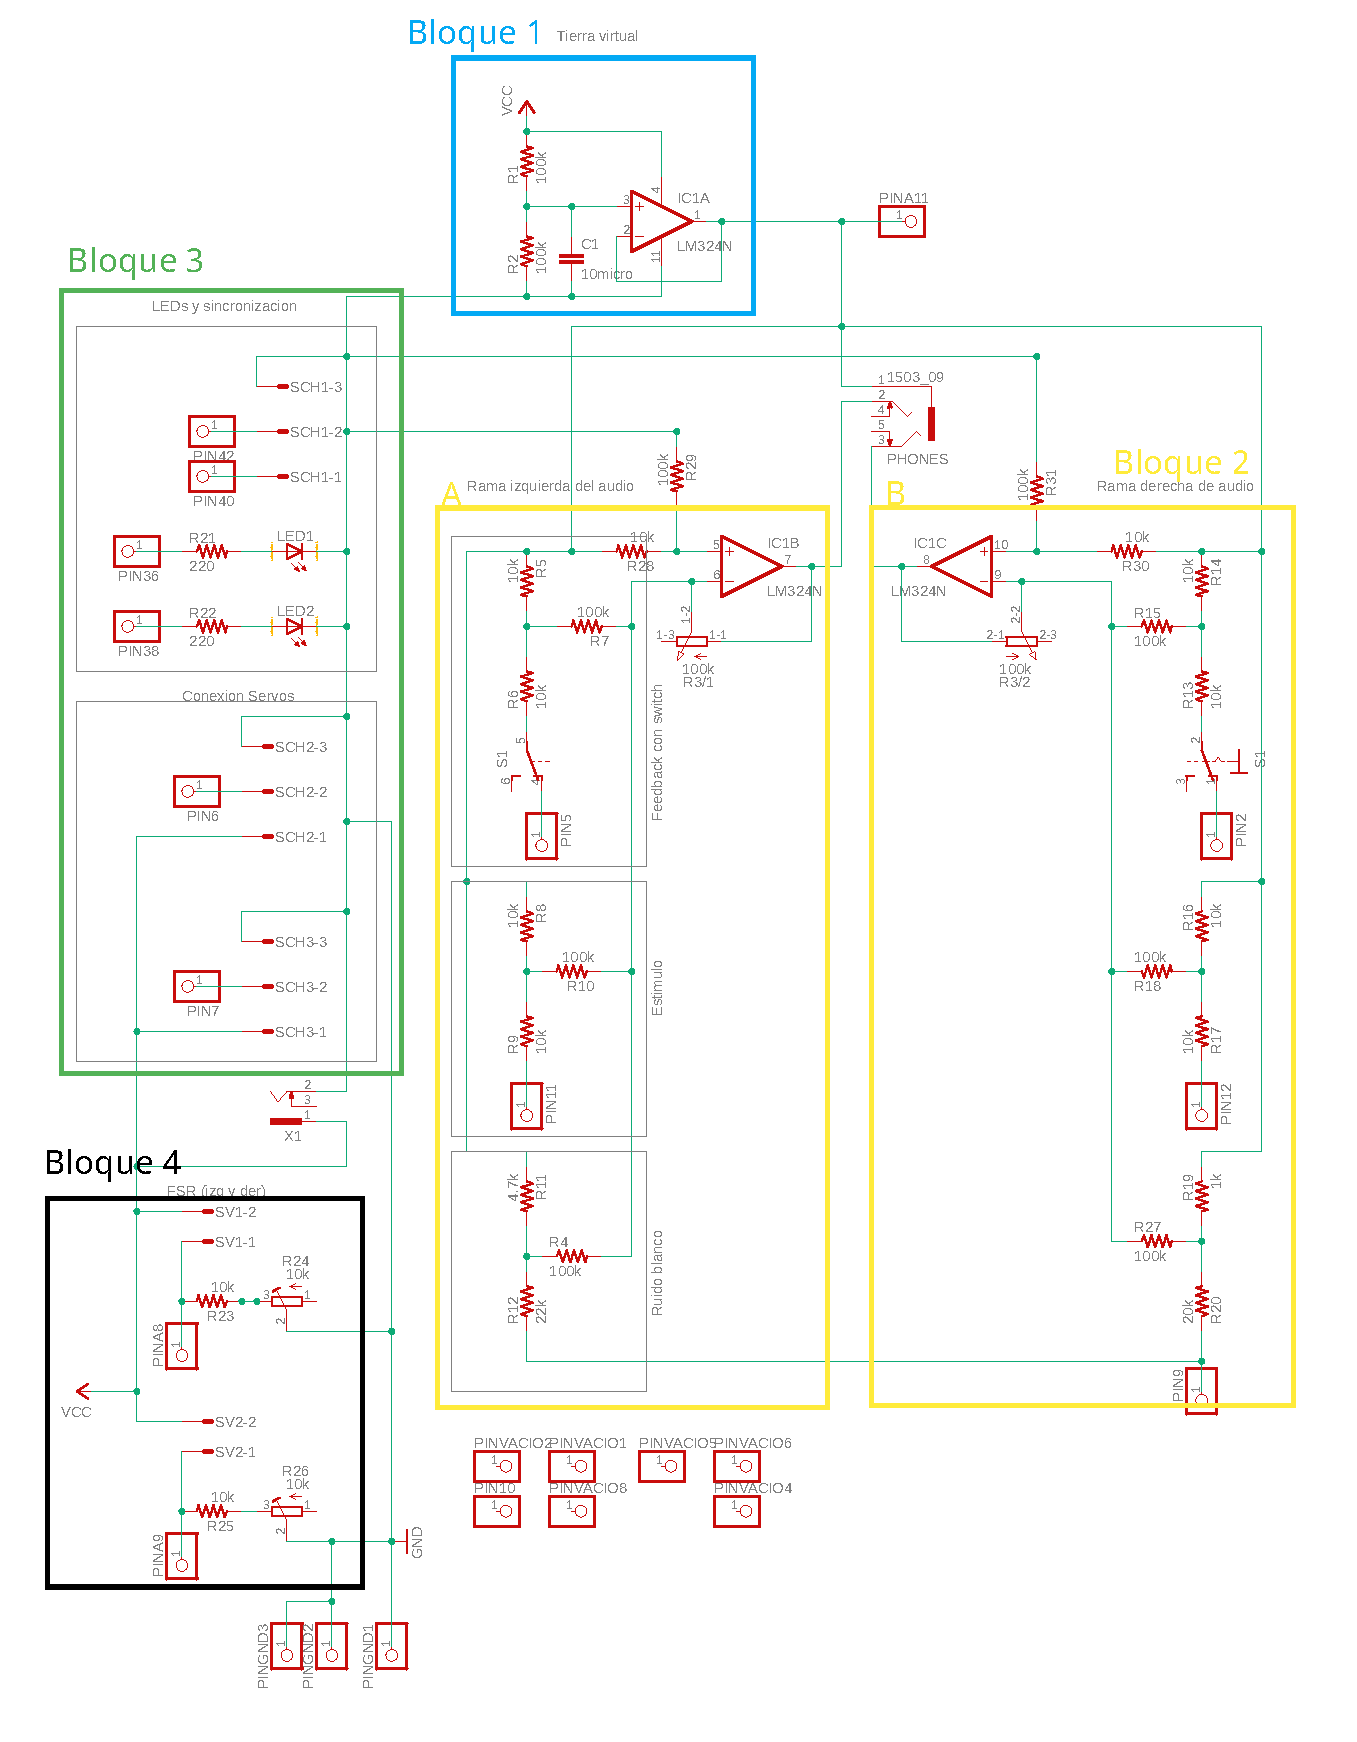
\includegraphics[width=0.8\linewidth]{figures/schematic.pdf}
    \caption{Circuit schematic. Block 1: virtual ground. Block 2: independent audio channels. Block 3: temporal alignment, visual stimuli, and servo driving. Block 4: force sensor connectors. Pin A11 is used as analog input to record the actual value of virtual ground and making it available to the code.}
    \label{fig.schematic}
\end{figure*}



\begin{figure*}[!ht]
    \centering
    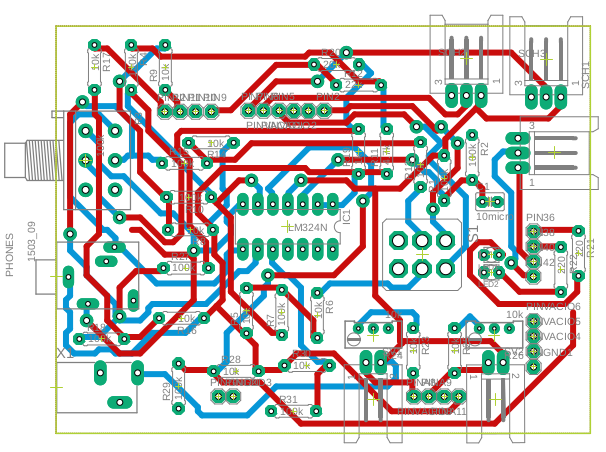
\includegraphics[width=0.7\linewidth]{figures/Circuito Tappingduino 3 Final - BRD ConexionCorrectaPower - CROP.png}
    \caption{PCB layout. Red traces: top layer, blue traces: bottom layer. Ground planes not shown.}
    \label{fig.BRDCompleto}
\end{figure*}





\subsection{PCB design}

Components were initially located based on a trade-off among several criteria: proximity to corresponding Arduino pins, proximity among related components, simplicity and accessibility for the user, and simplicity for soldering. We decided to use a double-sided copper-clad laminate. We took into account the following specific considerations:

\begin{description}
    \item[Soldering to a specific layer.] Some components have very short legs and are very difficult to solder to the layer where they sit due to potential damage to the component. For instance, in the top layer: switches, op amps sockets, potentiometers, female miniplug connectors, and trimpots; in the bottom layer: pins to connect to Arduino. That is why we constrained the auto-routing to prevent a trace to reach any of these components on the same layer (polygons in tRestrict and bRestrict in Eagle).
    
    \item[Forbidden regions for vias.] Vias are connections between the two copper layers. Components that sit close to the layer are difficult to solder when they have a via beneath them, so we defined polygons (vRestrict) to prevent the location of vias beneath components (other than regular resistors).
    
    \item[Central connector in Arduino.] Arduino Mega 2560 has a six-pin connector in the middle, so any soldering in the bottom layer could potentially make electrical contact with it. To avoid this we placed a bRestrict polygon thus preventing any component or connection to be located there.
    
    \item[Extra pins for better structural stability.] We added several pins with no electrical function in order to have a better union between Arduino and the shield.
    
    \item[Size of pads and vias.] To make drilling and soldering easier we increased the size of pads and vias.
    
    \item[Ground planes.] We covered empty spaces in both layers with polygons connected to ground for easier routing and reducing electrical noise and interference.
    
    \item[Isolation of vias.] Vias connected to the ground plane were termically isolated to prevent loss of heat during soldering.
    
    \item[Size of laminate.] The size of the copper-clad laminate was increased beyond the size of the Arduino to give Eagle a little more room to route traces.
\end{description}



Figure \ref{fig.BRDCompleto} shows the final design of the PCB. We attempted several different initial distribution of components and several auto-routings each, and chose the one that maximized the completion percentage and minimized the number of vias to simplify soldering. Figure \ref{fig.HardwareFinal} shows the actual finished shield.



\begin{figure*}[!ht]
    \centering
%    \includegraphics[width=0.75\linewidth]{figures/CircCollage_conCarteles.png}
    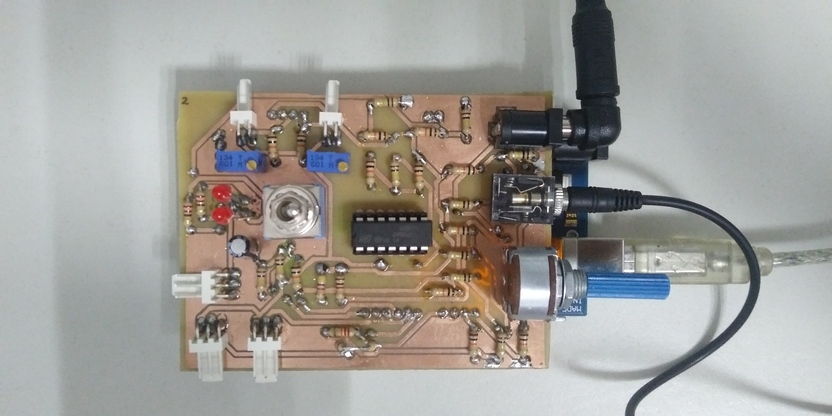
\includegraphics[width=0.75\linewidth]{figures/shield_fromabove.jpg}
    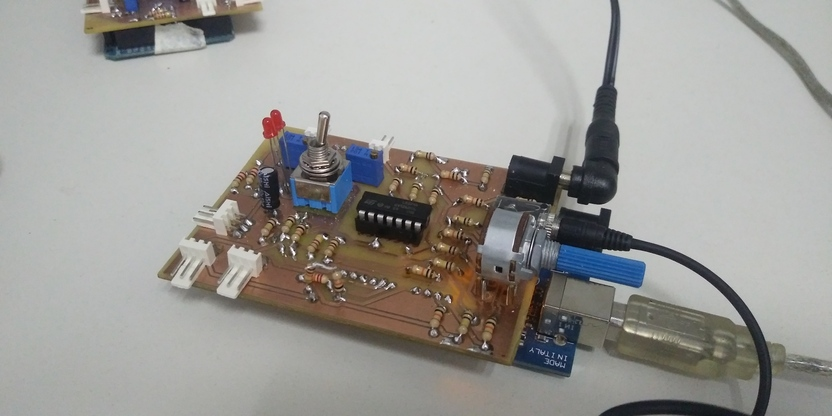
\includegraphics[width=0.75\linewidth]{figures/shield_angled.jpg}
    \caption{Actual finished shield, plugged on top of Arduino.}
    \label{fig.HardwareFinal}
\end{figure*}






\section{Software}

\subsection{Flow control}

The experimental unit in a typical finger tapping experiment is the trial, where the subject is exposed to a sequence of consecutive 30-45 brief stimuli. Trials are separated by pauses, and are grouped in blocks. A full experiment is a few blocks long.

The general control of flow during the experiment is performed by an experiment controller written in Python, while the control during a trial switches to the Arduino code in C. The experiment controller and the trial controller communicate to each other with text messages via the Serial port: the experiment controller sends the current trial parameters (interstimulus interval, number of stimuli, perturbation size, etc.), the trial controller records a trial and sends back the trial data (e.g. response times).



\subsection{Trial controller and Arduino timers}
\label{sec.timers}

We based our Arduino software development on Taparduino \cite{Schultz2016}.

One of the main functions of the Arduino-shield duo is producing sound, that is an analog voltage signal. However, the output pins in Arduino are only capable of having digital values (either HIGH or LOW), so a technique called pulse width modulation (PWM) is needed, where the pin is switched between HIGH and LOW at a high frequency with a variable duty cycle. The averaging over many oscillations leads to a continuous mean value depending on the duty cycle (close to LOW for a small duty cycle, or close to HIGH for a large duty cycle).

PWM is performed via timers, which are dedicated internal clocks/counters that operate in parallel with the central processor and can execute small portions of code on an interrupt basis. Timers in all operation modes work by counting from 0 through $2^b-1$, where $b$ is the number of bits of the timer, at a frequency $f_{\mbox{\scriptsize timer}} = 16\,\mbox{MHz}/2^b$, where 16 MHz is the oscillation frequency of the crystal in Arduino. Once counting reaches its TOP value it overflows and starts over again. The counting frequency can be modified by setting prescalers according to eq.\ \ref{ec.prescaling} \cite{arduinomanual}:
\begin{equation}
    f_{\mbox{\scriptsize timer}} = \frac{16\,\mbox{MHz}}{N \cdot 256}
    \label{ec.prescaling}
\end{equation}

\noindent Prescaler $N$ can take values $N=1,8,16,\dots$.

Every timer has two channels each associated with a different output pin, and can have different duty cycles. We used timers to generate sounds corresponding to stimuli and (optional) auditory feedback from the taps, and to generate masking noise. The appropiate timer configuration is known as FastPWM (with reset on overflow) and is shown in Figure \ref{fig.FastPWM} \cite{TimersOVF}.

\begin{figure}[ht]
    \centering
    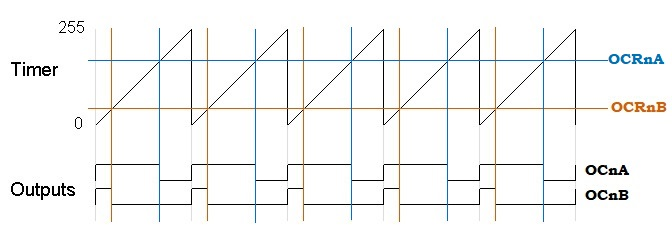
\includegraphics[width=\linewidth]{figures/FastPWM_cb.jpg}
    \caption{Timing diagram of a timer in 8-bit Fast PWM mode. The timer counts from 0 through 255 where it overflows and executes an interrupt. Registers OCRnA and OCRnB determine the duty cycle of each channel. Reproduced from \cite{TimersOVF}}
    \label{fig.FastPWM}
\end{figure}

We chose timers 1 and 3 for stimulus and feedback, respectively, and their channels A and B for left and right audio channels, respectively. Registers OCR1A and OCR1B determine the duty cycle of each channel in timer 1 (OCR3A and OCR3B for timer 3) and can be set independently. This allows us to send different audio signals to either ear. Timers 1 and 3 are 16-bit timers and can be set in 9-bit Fast PWM mode, which sets the interrupt frequency at approximately 31 kHz. This allows us to produce sound with an acceptable quality up to a fundamental frequency of around 2 kHz.

We used timer 2 to generate noise. Timer 2 has less resolution than timers 1 and 3 (it is an 8-bit timer) but quality is not as important in this case.


\subsection{Sound production}
\label{sec.sonido}

An analogous sound wave can be produced by a digital output by means of PWM: the digital output is switched between HIGH and LOW at a high frequency with a variable duty cycle, and then a low-pass filter with an appropriate cutoff frequency leads to a smoothed version of the signal whose mean value tracks the duty cycle \cite{arduinofading}. Figure \ref{fig.PWMsine} shows how a square wave with a time-varying duty cycle leads to a smooth low-pass filtered sinusoidal curve.

\begin{figure}[ht]
    \centering
    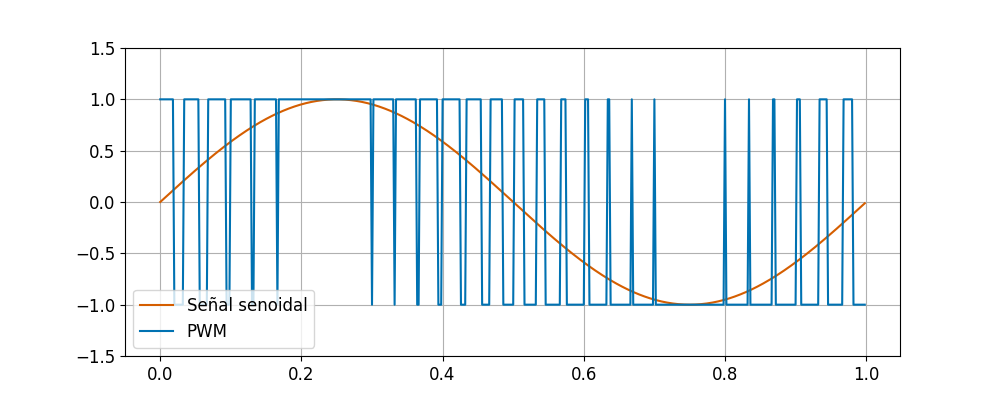
\includegraphics[width=\linewidth]{figures/EsquemaPWM.png}
    \caption{PWM with a relatively slowly varying duty cycle (blue curve) followed by low-pass filtering can produce a smooth sinusoidal signal with a well-defined frequency (orange curve).}
    \label{fig.PWMsine}
\end{figure}


The frequency of the sinusoidal is determined by the frequency of the duty cycle, and this in turn is set in the following way. Every time the timer overflows we set a new OCRnX value according to a lookup table with values that uniformly sample one period of the desired waveform, such that the duty cycle follows it. Figure \ref{fig.TablaSenoCompletay440} shows the contents of the lookup table for a sinusoidal waveform (orange curve). The actual frequency of the duty cycle (and thus of the sound signal) can be chosen by down- or up-sampling the lookup table. Down-sampling (by skipping values) leads to higher frequencies, while up-sampling (by repeating values) leads to lower frequencies. Either way can be detrimental to sound quality if excessive. When up-sampling, quality can be improved by interpolating (instead of just repeating values) but that would increase the load on the micro-controller so a trade-off analysis would be needed.

The blue curve in Figure \ref{fig.TablaSenoCompletay440} corresponds to down-sampling the lookup table to get a 440 Hz sinusoidal waveform. The lookup table is down-sampled by selecting values separated by a fixed quantity called the {\em frequency tuning word} (FTW):

\begin{equation}
    FTW = \frac{f_{\mbox{\scriptsize out}} \times 2^{32}}{f_{\mbox{\scriptsize timer}}}
\end{equation}

\noindent where $f_{\mbox{\scriptsize out}}$ is the desired output frequency in Hz, $2^{32}$ is the resolution of the phase accumulator, and $f_{\mbox{\scriptsize timer}}$ is the timer frequency in Hz \cite{ftw}.


\begin{figure}[ht]
    \centering
        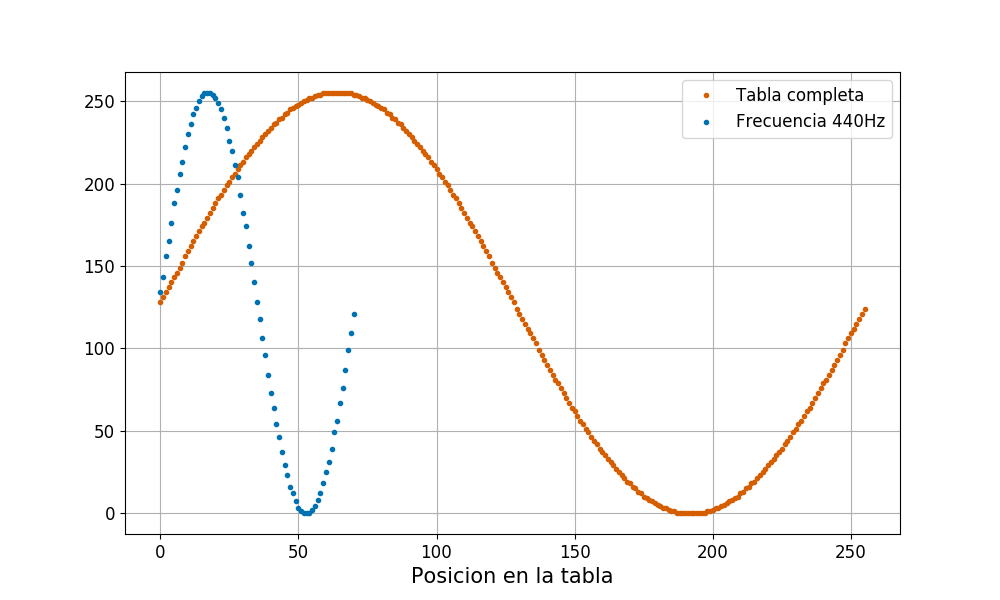
\includegraphics[width=\linewidth]{figures/Esquema_LUT_Sin.png}
        \caption{Contents of the lookup table for a sinusoidal waveform (orange), and down-sampling to a frequency of 440 Hz (blue).}
        \label{fig.TablaSenoCompletay440}
\end{figure}



\subsection{Noise generation}
\label{sec.noise}

We generate noise by randomly switching the PWM duty cycle such that the low-pass filtered signal randomly oscillates around virtual ground. A noise amplitude is defined with value up to half the TOP value of the timer, and a number of overflow periods is pseudorandomly chosen by a lightweight linear-feedback shift register \cite{galoisLFSR} (range 2-4). The duty cycle is set at a value equal to virtual ground + amplitude for the chosen number of periods, then reset to virtual ground - amplitude for the same number of periods, and then the number of periods is newly chosen to start over. In this way the noise power spectrum is relatively independent of the chosen amplitude.


\section{Open software and hardware}

Code for the experiment controller in Python and the trial controller in C, and .sch and .brd Eagle files for the circuit schematic and PSB are available in the following GitHub repository: \url{https://github.com/SMDynamicsLab/Tappingduino}.


\printbibliography


\end{document}



